\documentclass[a4paper,11pt, DIV=12]{scrartcl}
\usepackage[utf8x]{inputenc}

\usepackage{graphics} % for pdf, bitmapped graphics files
\usepackage{epsfig} % for postscript graphics files
\usepackage{amsmath} % nicer formulas
\usepackage{amssymb}  % some additional symbols.
\usepackage{amsfonts}
\usepackage{booktabs} % nicer tabular
\usepackage{biblatex}
\usepackage{hyperref}
\usepackage{caption}
\usepackage{subcaption}
\usepackage{array}
\usepackage{adjustbox}

\allowdisplaybreaks
\addbibresource{sources.bib}

\newcommand{\x}{\boldsymbol{x}}
\newcommand{\y}{\boldsymbol{y}}
\newcommand{\vp}{\boldsymbol{v}^+}
\newcommand{\vm}{\boldsymbol{v}^-}
\newcommand{\ve}{\boldsymbol{v}}

\title{Examination of Unpaired Translation Methods for Near-Infrared Image Colorization}
\author{Ayk Borstelmann\footnote{student id number: 3441004, address: Koenigswinterer Str. 204, 53227 Bonn}}

\begin{document}

\maketitle

\section{Introduction}

\subsection{Related Work}

% For paired NIR -> RGB image translation: pixel to pixel registration % temporal synchronization  

% Work in the Supervised Setting (Paired Image Translation)

% Why using Unpaired Image Translation in the first place ? 

\section{Dataset}
While examining both proposed methods for their suitability for near-infrared colorization multiple datasets
and two data sources were used \textit{Caltech Camera Traps} and \textit{Snapshot Serengeti} due to advantages
and disadvantages of those.

\subsection{Caltech Camera Traps}
\textit{Caltech Camera Traps} (CCT) is a dataset consisting of $243.100$ images from $140$ camera locations
in the southwestern united states with $21$ animal label categories \cite{caltech}.
In particular, it also contains near-infrared images mostly at night and regular RGB images in the daytime.
Approximately $70 \%$ of the overall image set is labeled as empty.
Annotations are provided in the \textit{COCO Camera Traps} format describing meta information via JSON \cite{caltech}
This allows an automatic parsing of the available images as well as efficient access to information about
the images which comes in useful when creating sub-datasets for training networks.
Unfortunately, the COCO format does not provide information on whether the image is an RGB- or a NIR image.

\subsection{Snapshot Serengeti}
In contrast to the CCT dataset, \textit{Snapshot Serengeti} is a much larger dataset and comes from the Snapshot Serengeti National Park in Tanzania.
It consists of $7.1$ million images through seven seasons of the Snapshot Serengeti Project \cite{serengeti}.
There are $61$ labeled species where as approximately $76\%$ of the images are labeled as empty.
Similar to the CCT dataset, Snapshot Serengeti contains near-infrared images as well as RGB images and
is annotated in the COCO Camera Traps format \cite{serengeti} and therefore is an easy addition to the CCT dataset.
In contrast to the CCT dataset, it contains also many RGB images from nighttime using incandescent lightning which
proves handy for the training of NIR to RGB translation.

\subsection{Subset Generation}
Since both datasets (CCT and Snapshot Serengeti) are substantially larger than processable for training,
choosing a subset of those images is essential. The requirements for this subset strongly influence the performance
of the models.

1. For both suggested models the input dataset needs to be divided into input- and output-domain, NIR and RGB.
2. To gain model performance in the main objective, which is colorizing NIR images of animals,
choosing only images that contain animals is important.
3. Training with a variety of image locations proves to decrease the overfitting for the translation
and therefore a uniform distribution of the available locations should be approximated.
4. Since most NIR images are taken at night the network should not be influenced to solve the more difficult
task of translating images from NIR night to RGB day. This can be archived by only allowing night images for both
domains.

The 2., 3. and 4. requirements are all archivable by using the provided information from the COCO format and therefore
are already defined before downloading a single image.
While only choosing images with animals is done by a simple filter on the dataset before sampling the approximately uniform distribution
of locations can be archived using a weighted sampling where the weight is the inverse of the location occurrences.
The COCO format also documents the time of recording. This can be used to only sample images from the night.
Using the timezones and the geolocations where the datasets were recorded, individual time frames for each day of the year can serve as filters for night images.

Since the COCO format does not provide information about which item is a NIR- and which item is an RGB image \cite{caltech}, that information is not obtainable before downloading.
Because both datasets provide their NIR images with \textit{colored} logos, they are stored in an RGB image where the actual image section has equal values over all three channels.
Therefore a simple solution is the download the images and compare the three channels in a cropped version of the image.

This whole process can be automated in the form of a mix between a rejection- and an importance sampler. It samples from the filtered dataset with weights by location, downloads the image and
rejects a sample if the desired size of NIR- or RGB images is already reached.
Finally, the produced subset can be stored in a compact format to archive reproducibility across systems.

\section{Proposed Methods}

For image translation, a mapping function $G: \mathcal{X} \to \mathcal{Y}$ shall be learned.
In our case, $\mathcal{X}$ is the input domain of Near-Infrared images whereas $\mathcal{Y}$ is the output domain of colored RGB images.
For the training a dataset of unpaired images sets $X = \{\x \in \mathcal{X}\}$, $Y = \{\y \in \mathcal{Y}\}$ is given.
For the unpaired image translation, the mapping function must be learned without any existing $\x \in X$ for which $G(\x)=\y$ is known.
Therefore supervised learning techniques are not applicable and unsupervised learning methods should be used.

\textit{Generative Adversarial Networks} (GANs) provide a way of learning this function by declaring the objective that for a $\x \in \mathcal{X}$, $G(\x) = \hat{\y}$
should be indistinguishable from images out of $\y \in \mathcal{Y}$. GANs achieve this by splitting the training architecture into two networks:
The \textit{generator} $G: \mathcal{X} \to \mathcal{Y}$ that learns the relationship between the two domains and the \textit{discriminator} $D: \mathcal{Y} \to \mathbb{R}$ which learns to
classify possible images from $Y$ as "real" or "generated".
Both networks optimize each other and play a min-max game:
The generator tries to fool the discriminator into classifying the generated image as "real" and thereby learns to produce \textit{indistinguishable} images from $Y$.
Additionally, the discriminator tries to detect generated images accordingly and also learns the features of the domain $Y$ by classifying those as "real".

Although this method has already proven to perform well for image translation, %TODO source
it has issues keeping the content. GANs in general are not restricted in the training to mapping the actual \textbf{content} from the given image
$\x \in X$ to the produced image $G(\x) \in Y$.
E.g. one could imagine that for a given $\y \in Y$ the mapping function which maps all $\x$ to a fixed $\y$ ($G(\x) = \y$)
should perform exceptionally well considering its training loss because the produced image is always classified as "real".
This case is called \textit{mode collaps} and can be weakened by adding additional structure to the training.

In the following, we will concentrate on two options:
1. Using a \textit{cycle consistency loss} which was introduced by Zhu \textit{et. al.} for the network \textit{CycleGAN} \cite{cyclegan_orig}
and 2. using a \textit{contrastive loss} which was introduced into this setting by Park \textit{et. al.} for the network \textit{CUT} \cite{cut}.

\subsection{CycleGAN}
CycleGAN is network architecture presented by Zhu \textit{et. al.} and introduces a \textit{cycle consistency loss} for image translations using GANs.
The idea is that the translation between the two domains should be "cycle consistent" meaning that when we translate an image from NIR to RGB and then back
to NIR both NIR images should be approximately equal.
Mathematically this means if we have an additional function $F: \mathcal{Y} \to \mathcal{X}$ which is the approximately inverse of $G$ then for a $\x \in \mathcal{X}$, $F(G(\x)) \approx \x$
which is encouraged by a \textit{cycle consistency loss} \cite{cyclegan_orig}. We assume that if a $\x$ is recoverable from a $\y = G(\x)$ using $F$ then the content of $\x$
is preserved in $\y$ \cite{cyclegan_orig}.

\subsubsection*{Cycle Consistency Loss}
We can write this objective into a loss function $\mathcal{L}_{cyc}(G, F)$ which uses an L1 norm to encourage cycle consistency (\autoref{eqn:cyc}).
In addition to the already mentioned \textit{forward cycle consistency}, CycleGAN also utilizes \textit{backward cycle consistency} meaning that for a $\y \in \mathcal{Y}$
also $G(F(\y)) \approx \y$ \cite{cyclegan_orig} should be.

\begin{equation}
   \label{eqn:cyc}
   \begin{aligned}
      \mathcal{L}_{cyc}(G, F) = \underbrace{\mathbb{E}_{\x \sim X}\left[||F(G(\x)) - \x||_1\right]}_{\text{forward cycle consistency}} +
      \underbrace{\mathbb{E}_{\y \sim Y}\left[||G(F(\y))) - \y||_1\right]}_{\textit{backward cycle consistency}}
   \end{aligned}
\end{equation}

In addition to the L1 cycle consistency loss, Mehri \textit{et. al.} propose to use SSIM as a second cycle consistency loss \cite{mehri2019colorizing}.
Contrary to the L1 loss, the \textit{structural similarity index} measures the differences between the images not by the absolute image intensity values but
by comparing two images based on luminance-, contrast- and structural similarity \cite{ssim}.

Using measurements for luminance $l(\y_1, \y_2)$, contrast $c(\y_1,\y_2)$ and structure comparison $s(\y_1, \y_2)$ we can obtain the overall structural similarity
index $SSIM(\y_1, \y_2)$ as multiplication of each component (\autoref{eqn:ssim}) \cite{ssim}.

\begin{equation}
   \label{eqn:ssim}
   \begin{aligned}
      SSIM(\y_1, \y_2) = l(\y_1, \y_2) \cdot c(\y_1,\y_2) \cdot s(\y_1, \y_2)
   \end{aligned}
\end{equation}

The SSIM is obtained using a moving gaussian window over the image and therefore the SSIM difference between two images $\overline{SSIM(\y_1,\y_2)}$ is calculated as follows (\autoref{eqn:ssim_difference}).
We denote $\y_{1,j}$ and $\y_{2,j}$ as the image contents of the $j$-th local patch using the gaussian window whereas $M$ is the number of gaussian windows.

\begin{equation}
   \label{eqn:ssim_difference}
   \begin{aligned}
      \overline{SSIM(\y_1,\y_2)} = \frac{1}{M}\sum_{j=1}^{M}1 - SSIM(\y_{1,j},\y_{2,j})
   \end{aligned}
\end{equation}

Finally the cycle consistency loss $\mathcal{L}_{SSIM}(G,F)$ can be constructed using the differences in the SSIMs between the images (\autoref{eqn:ssim_loss}).

\begin{equation}
   \label{eqn:ssim_loss}
   \begin{aligned}
      \mathcal{L}_{SSIM}(G,F) & = \mathbb{E}_{\x \sim X}\left[\overline{SSIM(F(G(\x)), \x)}\right] + \mathbb{E}_{\y \sim Y}\left[\overline{SSIM(G(F(\y)), \y)}\right] \\
                              & = \mathbb{E}_{\x \sim X}\left[\frac{1}{M}\sum_{j=1}^{M}1 - SSIM(\x_{1,j},\x_{2,j})\right] +
      \mathbb{E}_{\y \sim Y}\left[\frac{1}{M}\sum_{j=1}^{M}1 - SSIM(\y_{1,j},\y_{2,j})\right]
   \end{aligned}
\end{equation}


\subsubsection*{Relativistic Adversarial Loss}
For both generators, adversarial discriminators $D_X$ and $D_Y$ are introduced where $D_X$ has the aim of distinguishing between real images
$X$ and generated images $\{F(\y)\}$ and $D_Y$ for $Y$ and $\{G(\x)\}$.
For both, we apply a relativistic GAN loss namely \textit{RaLSGAN} \cite{mehri2019colorizing,rel_gan}.
\autoref{eqn:ralsgan} demonstrates the RaLSGAN loss for the generator $G$ ($\mathcal{L}^G_{RaLSGAN}(G,D_Y,X,Y)$) and its discriminator
$D_Y$ ($\mathcal{L}^D_{RaLSGAN}(G,D_Y,X,Y)$), the loss for $F$ and $D_X$ is defined analogous \cite*{rel_gan}.

\begin{equation}
   \label{eqn:ralsgan}
   \begin{aligned}
      \mathcal{L}^{D_Y}_{RaLSGAN}(G,D_Y,X,Y) & = \mathbb{E}_{\y \sim Y}\left[(D_Y(\y) - \mathbb{E}_{\x \sim X} D_Y(G(\x)) - 1)^2 \right] \\
                                             & + \mathbb{E}_{\x \sim X}\left[(D_Y(G(\x)) - \mathbb{E}_{\y \sim Y} D_Y(\y) + 1)^2 \right] \\
      \mathcal{L}^G_{RaLSGAN}(G,D_Y,X,Y)     & = \mathbb{E}_{\x \sim X}\left[(D_Y(G(\x)) - \mathbb{E}_{\y \sim Y} D_Y(\y) - 1)^2 \right] \\
                                             & + \mathbb{E}_{\y \sim Y}\left[(D_Y(\y) - \mathbb{E}_{\x \sim X} D_Y(G(\x)) + 1)^2 \right]
   \end{aligned}
\end{equation}

\subsection*{Identity Loss}
Lastly, the identity loss function has the aim of regulating the generator:
If an image already looks like a colored RGB image, it should not be modified.
This leads to the identity loss $\mathcal{L}_{identiy}$ (\autoref{eqn:identity_loss}) \cite{mehri2019colorizing}.

\begin{equation}
   \label{eqn:identity_loss}
   \begin{aligned}
      \mathcal{L}_{identiy}(G, F) = \mathbb{E}_{\x \sim X} \left[||G(\x) - \x||_1\right] + \mathbb{E}_{\y \sim Y} \left[||G(\y) - \y||_1\right]
   \end{aligned}
\end{equation}

\subsection*{Full Objective}
All those four loss functions lead to an additive final loss function (\autoref{eqn:cycle_gan_total_loss}) \cite{mehri2019colorizing}.
$\lambda$ and $\gamma$ are weights for the relative importance of the L1 cycle consistency loss and the identity loss.

\begin{equation}
   \label{eqn:cycle_gan_total_loss}
   \begin{aligned}
      \mathcal{L} = \lambda \mathcal{L}_{cyc} + \mathcal{L}_{SSIM} + \gamma \mathcal{L}_{identity}(G,F) + \mathcal{L}_{RaLSGAN}^G(G,D_Y,X,Y) + \mathcal{L}_{RaLSGAN}^F(F,D_X,Y,X)
   \end{aligned}
\end{equation}

\subsubsection*{U-Net}
In praxis, both functions $G$ and $F$ are generation networks. In contrast to ResNet generators \cite{resnet} Zhu \textit{et al} used in the original CycleGAN \cite{cyclegan_orig}
U-Net generators \cite{unet} proposed by Mehri \textit{et. al.} are used, because they perform better in learning the color without affecting the image shape \cite{mehri2019colorizing}.
Additionally, U-Net generators also need less computational time compared to Resnet \cite{mehri2019colorizing}.

\subsubsection*{Optimizations}
\begin{enumerate}
   \item TTUR
   \item Spectral Normalization
   \item Decrease Cycle Consistency weight $\lambda$ over time
\end{enumerate}


\subsection{Contrastive Unpaired Translation (CUT)}
CycleGAN solves the content preservation using a cycle consistency loss which requires duplication of the architecture
of the GAN to have an inverse and also assumes a bijection between the $\mathcal{X}$ and $\mathcal{Y}$ \cite{cyclegan_orig}.
The network is forced to learn a revertable translation and therefore some freedom for realistic appearance may be lost.
CUT on the other hand doesn't require the learned function $G$ to be invertible.
It encourages content preservation by requiring a patch from the output image, e.g. a wildebeest's leg to be most likely to also come from that patch
of the input image and not from somewhere else in the image, e.g. the trees in the background. \cite{cut} This is called patchwise contrastive learning.

\subsubsection*{Patch NCE Loss} % what does NCE stand for ? 
First given a patch of the output image referenced as "query", we want to maximize the probability that the corresponding
patch from the input image, referenced as "positive", would be associated with the query over other input patches referenced
as "negatives".
The query, the positive and the $N$ negatives are represented by $K$-dimensional vectors, $\ve \in \mathbb{R}^K$, $\vp \in \mathbb{R}^K$
and $\vm_n \in \mathbb{R}^K$ as the $n$-th negative and $\ve_n^- \in \mathbb{R}^{N \times K}$.
Then we can define a cross-entropy loss $l(\ve, \vp, \vm)$ for $\vp$ being associated over $\vm_n$ (\autoref{eqn:patch_loss}).
Note Park \textit{et. al.} added a scaling of $\tau = 0.007$ and normalized the vectors into a unit sphere \cite{cut}.

\begin{equation}
   \label{eqn:patch_loss}
   \begin{aligned}
      l(\ve, \vp, \vm) = - \log \left[ \frac{\exp(\ve \cdot \vp / \tau)}{\exp(\ve \cdot \vp / \tau) + \sum_{i=1}^N\exp(\ve \cdot \ve_n^- / \tau)}\right]
   \end{aligned}
\end{equation}

To obtain those patch representations as $K$-dimensional vectors Park \textit{et. al.} proposed to use the already existing
generator function $G$. $G$ is an encoder-decoder network, therefor $G(\x) = G_{dec}(G_{enc}(\x))$, where $G_{enc}$ denotes the encoder \cite{cut}.
Each layer of the encoder network represents multiple patches of the input images. To map this layer to condensed feature vectors,
a small Multi-Layer-Perception $H_l$ with 2 layers is used, where $H_l$ maps the $l$-th layer of the encoder network to features
$\boldsymbol{z}_l \in \mathbb{R}^{S_l \times C_l}$, therefore $\boldsymbol{z}_l = H_l(G_{enc}^l(\x))$.
$S_l$ is the number of spatial locations and $C_l$ is the size of each feature vector.
For each layer of interest $l \in \{1, \dots, L\}$ the spatial location $s \in \{1, \dots S_l\}$ inside the layer represents a patch of the input image.
We denote $\boldsymbol{z}_l^s \in \mathbb{R}^{C_l}$ as the feature corresponding to the spatial location which therefore is a vector representation of a patch
in the input image. All other features of patches in the images are referred to as $\boldsymbol{z}_l^{S \setminus s} \in \mathbb{R}^{(S_l - 1) \times C_l}$
As we now have input image patches we additionally need output query patches as features. Using the same mechanism on the output image we can obtain
$\boldsymbol{\hat{z}}_l = H_l(G_{enc}^l(G(\x)))$. Using the loss defined in \autoref{eqn:patch_loss}, we can obtain a loss for the content preservation of the
GAN $\mathcal{L}_{PatchNCE}(G,H,X)$ \autoref{eqn:patchnce_loss} \cite{cut}.

\begin{equation}
   \label{eqn:patchnce_loss}
   \begin{aligned}
      \mathcal{L}_{PatchNCE}(G,H,X) = \mathbb{E}_{\x \sim X} \sum_{l = 1}^L \sum_{s=1}^{S_l} l(\boldsymbol{\hat{z}}_l^s, \boldsymbol{z}_l^s, \boldsymbol{z}_l^{S \setminus s})
   \end{aligned}
\end{equation}

\subsubsection*{Identity Loss}
Additionally to the $\mathcal{L}_{PatchNCE}(G, H, X)$ which is applied on the input images, Park \textit{et. al.} propose to use the loss on the output dataset too,
which is a form of identity loss, specific to the domain \cite{cut}.

\subsection*{Adversarial Loss}
The adversarial loss as the GAN objective is an SGAN loss therefore $\mathcal{L}_{GAN}(G, D, X, Y)$ is defined
as follows (\autoref{eqn:cut_gan}) \cite{cut}.

\begin{equation}
   \label{eqn:cut_gan}
   \begin{aligned}
      \mathcal{L}_{GAN}(G, D, X, Y) = \mathbb{E}_{\y \sim Y}\log(D(\y)) +  \mathbb{E}_{\x \sim X}\log(1 - D(G(\x)))
   \end{aligned}
\end{equation}

\subsubsection*{Full objective}
The final objective $\mathcal{L}$ for the CUT network is then as follows (\autoref{eqn:cut_total_loss})) \cite{cut}.

\begin{equation}
   \label{eqn:cut_total_loss}
   \begin{aligned}
      \mathcal{L} = \mathcal{L}_{GAN}(G, D, X, Y) + \mathcal{L}_{PatchNCE}(G,H,X) + \mathcal{L}_{PatchNCE}(G,H,Y)
   \end{aligned}
\end{equation}

\section{Evaluation}
The two main application contexts of NIR image colorization are to increase human users' orientation for images taken with NIR cameras
and also to improve object recognition results due to the gained color information. We evaluate the two models using those two applications contexts:
We define qualitative evaluation categories focused on how natural the generated images look. Additionally, quantitative evaluation metrics to measure
the quality of the images regarding the two main application contexts (FID and classification performance) are used.

\subsection{Quantitative Evaluation Metrics}
Due two the unpaired setting also in the quantitative evaluation, classic solutions like the difference between absolute intensity values or the SSIM
\cite{ssim} cannot be applied. Fortunately, methods to compare the general image similarity of two sets like the FID \cite{ttur} or
comparing classification results using an off-the-shelf network are well-known to evaluate quantitatively the quality of the image translation.

\subsubsection*{FID}
To measure how near the generated images are real images regarding human perception the \textit{Fréchet Inception Distance} (FID) \cite{ttur} is a commonly used metric.
It empirically estimates how the human eye percepts images for a set of images and computes the distance between two such set representations.
First, a pretrained InceptionV3 model evaluates each image of the image set and the activation of the last layer is taken as the "human perception approximation".
Then for all activation vectors of the evaluated images in the images set, a multi-dimensional Gaussian is fitted over those activation vectors.
This is done for two image sets and then the two Gaussians are compared using the Fréchet Distance \cite{ttur}.
Intuitively, if the generated images are realistic, then the statistics of features in a classification network should be similar to the real ones.

\subsubsection*{Classification Results}
To satisfy the second application context generated images may improve classification results this can also be taken into account as a quantitative metric.

%TODO finish

\subsection{Qualitative Evaluation Methods}
As qualitative evaluation

%TODO define

\subsection{Dataset Evaluation}
Besides comparing both translation methods, a study on what are important points for generating subsets as well as the suitability of each parent dataset
(CCT and Snapshot Serengeti) as train datasets were done.


\begin{figure}[h]
   \centering
   \begin{tabular}[width=.1\textwidth]{c c}
      \textbf{NIR} \cite{caltech}                                                             & \textbf{Random} \\
      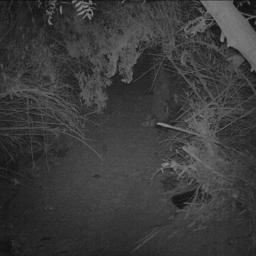
\includegraphics[width=.2\textwidth]{img/5858c26e-23d2-11e8-a6a3-ec086b02610b_real.png} &
      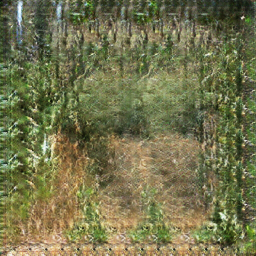
\includegraphics[width=.2\textwidth]{img/5858c26e-23d2-11e8-a6a3-ec086b02610b_hal.png}                    \\

      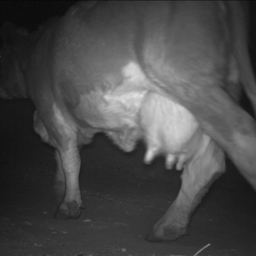
\includegraphics[width=.2\textwidth]{img/586936d3-23d2-11e8-a6a3-ec086b02610b_real.png} &
      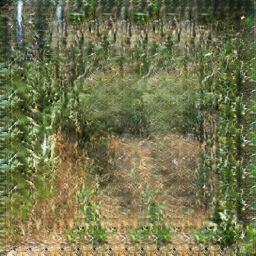
\includegraphics[width=.2\textwidth]{img/586936d3-23d2-11e8-a6a3-ec086b02610b_hal.png}
   \end{tabular}
   \caption{
      \textbf{Qualitative Evaluation.} Hallucination \& Mode Collaps because of \textit{dominant location occurrences}.
      \textbf{Random}: CycleGAN trained location independent sampled CCT dataset.
   }
   \label{fig:hallucincation-location}
\end{figure}

Firstly, it proved to be important to not only uniform sample from a dataset to generate a subset but to take the location occurrence into account.
Both datasets have a set of locations that dominate the dataset and therefore can substantially influence the training.
Mode collapse such that specific features of a location are generated independently of whether they are in the input image or not are
observable results (\autoref{fig:hallucincation-location}). An weighted sampling based on the location can solve this problem.


\begin{figure}[h]
   \centering
   \begin{subfigure}[h]{0.3\textwidth}
      \centering
      \begin{tabular}{l | c}
         Train Dataset       & FID $\downarrow$ \\
         \hline \hline
         \textbf{Random}     & 203.15           \\
         \textbf{Only Night} & 149.51
      \end{tabular}
      \caption{
         \textbf{Quantitative Evaluation.} FID between RGB CCT test dataset and generated RGB using CCT NIR test dataset as input for each network (\textbf{Random}, \textbf{Only Night})
      }
      \label{fig:hallucation-night-day-quan}
   \end{subfigure}
   \hfill
   \begin{subtable}[h]{0.65\textwidth}
      \centering
      \begin{tabular}{c c c}
         \textbf{NIR} \cite{caltech}                                                             & \textbf{Random} & \textbf{Only Night} \\

         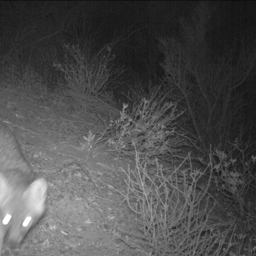
\includegraphics[width=.3\textwidth]{img/586ae0f6-23d2-11e8-a6a3-ec086b02610b_real.png} &
         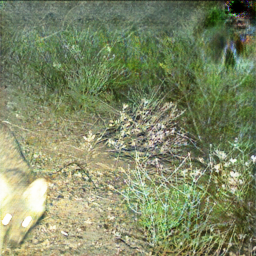
\includegraphics[width=.3\textwidth]{img/586ae0f6-23d2-11e8-a6a3-ec086b02610b_hal.png}  &
         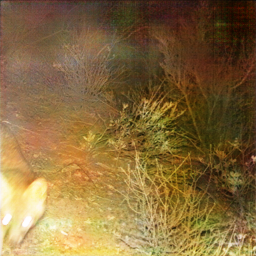
\includegraphics[width=.3\textwidth]{img/586ae0f6-23d2-11e8-a6a3-ec086b02610b_without_hal.png}                                  \\

         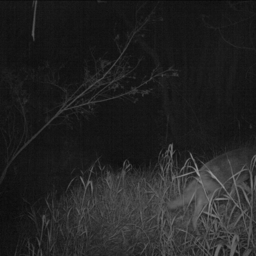
\includegraphics[width=.3\textwidth]{img/588c13ba-23d2-11e8-a6a3-ec086b02610b_real.png} &
         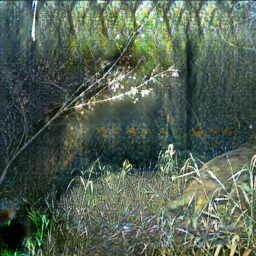
\includegraphics[width=.3\textwidth]{img/588c13ba-23d2-11e8-a6a3-ec086b02610b_hal.png}  &
         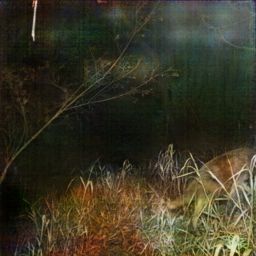
\includegraphics[width=.3\textwidth]{img/588c13ba-23d2-11e8-a6a3-ec086b02610b_without_hal.png}
      \end{tabular}
      \caption{
         \textbf{Qualitative Evaluation.} Evaluation of the two networks \textbf{Random}, \textbf{Only Night} on the CCT test dataset NIR images \cite{caltech}.}
      \label{fig:hallucation-night-day-qual}
   \end{subtable}
   \caption{
      Comparison of two training datasets used to train CycleGAN: Hallucination because of \textit{unintended night-to-day translation}.
      \textbf{Random}: CycleGAN trained on time independent sampled dataset of NIR images,
      \textbf{Only Night}: CycleGAN trained on only night NIR and RGB images (using Snapshot Serengeti dataset \cite{serengeti}).
   }
   \label{fig:hallucincation-night-day}
\end{figure}

Secondly, just providing random NIR and RGB for training also proved to be not optimal.
Commonly, camera traps take NIR images at night and RGB images during the day.
Therefore when sampling random NIR and RGB images, the Near-Infrared images are mostly from the night and the RGB images from the day.
This leads to the discriminator anticipating real RGB images to have daylight features such that the far points in the image are still visible as well as that the sky should be visible and preferably blue/gray.
Consequently, the generator tries to satisfy the discriminator and invents those features while translating.
Because night images don't have the information for those features the network invents them.
This effect is called \textit{hallucination}. It results in a substantial FID increase (\autoref{fig:hallucation-night-day-quan}) and the invention of information as
well as artifacts in the output image (\autoref{fig:hallucation-night-day-qual}).
This problem can be solved by only using night images for training (\textbf{Only Night} in \autoref{fig:hallucation-night-day-qual}).

% TODO find a better section for this discussion
Using the given timestamps on the COCO metadata of the CCT dataset \cite{caltech} a sampling of only night images failed due to too less RGB night images.
Snapshot Serengeti on the other hand used two cameras types during the survey:
Scoutgard's SG565 cameras which produce RGB \textbf{night} images using an \textit{incandescent} flash and
DLC Covert II cameras which use an infrared flash and therefore produce NIR night images \cite{serengeti}.
Therefore the Snapshot Serengeti Dataset is preferable to the CCT dataset as a training dataset for NIR to RGB night translation.

\subsection{Suitability of CUT}
While comparing CUT and CycleGAN it was noticed that CUT performed worse when trained on a NIR night to RGB day dataset than CycleGAN \autoref{TODO}.
It was \textit{hypothesized} that due to the contrastive loss of CUT which tries to assign patches from the output image the corresponding patch from the input image
\textit{in contrast} to other patches from the input image, CUT is not that well suited to do whole image translation, especially those laking distinct feature like
the NIR to RGB translation compared to partial image translation like translating images from a horse to a zebra as done by Park \textit{et. al.} \cite{cut}.
For example, it might be easier to assign such distinct parts as a horse head to a zebra head compared to assigning a colored scrub in the background exactly it's
corresponding NIR patch.

\begin{figure}[h]
   \centering
   \begin{adjustbox}{width=1\textwidth}
      \begin{tabular}{l | >{\centering\arraybackslash} p{5.5cm} | >{\centering\arraybackslash} p{3cm} | >{\centering\arraybackslash} p{3.5cm} }
         Model                                                  &
         Cityscapes (Semantic $\rightarrow$ Image) \newline FID $\downarrow$ &
         Horse $\rightarrow$ Zebra \newline FID $\downarrow$    &
         Winter $\rightarrow$ Summer \newline FID $\downarrow$                          \\
         \hline
         CycleGAN \cite{cyclegan_orig}                          & 75.97 & 76.37 & 86.14 \\
         CUT \cite{cut}                                         & 57.16 & 45.33 & 80.25
      \end{tabular}
   \end{adjustbox}
   \caption{
      Quantitative Comparison (FID) of CUT and CycleGAN for multiple datasets \cite{monce}.
      Horse $\rightarrow$ Zebra translates images of horses to zebras without changing the environment or posture of the animal (partial image translation).
      Cityscape (Semantic $\rightarrow$ Image) generates an image of a street based on semantic images of it (whole image translation with many distinct features).    
   }
   \label{}
\end{figure}



\section{Discussion}
\subsection{Comparison CUT vs CycleGAN}

\section{Conclusion}
\section{Future Work}
\section{Appendix}

\printbibliography

\end{document}

